\documentclass{book}
\usepackage{amsmath}
\usepackage{amssymb}
\usepackage{bm}
\usepackage{graphicx}
\usepackage{epstopdf}
\usepackage[bw]{mcode}
\usepackage{listings}
\DeclareGraphicsRule{.tif}{png}{.png}{`convert #1 `basename #1 .tif`.png}
\usepackage{color}
\pagestyle{plain}
%\pagestyle{empty}
\textheight 9 true in
\textwidth 6.5 true in
\hoffset -.75 true in
\voffset -.75 true in

\mathsurround=2pt  \parskip=2pt
\def\crv{\cr\noalign{\vskip7pt}}
\def\a{\alpha } \def\b{\beta } \def\d{\delta } \def\D{\Delta } \def\e{\epsilon }
\def\g{\gamma } \def\G{\Gamma} \def\k{\kappa} \def\l{\lambda } \def\L{\Lambda }
\def\th{\theta } \def\Th{\Theta} \def\r{\rho} \def\o{\omega} \def\O{\Omega}
\def\ve{\varepsilon}
\def\sech{\text{sech}}
\def\p{\partial}
\def\erf{\text{erf}}

\def\sA{{\cal A}} \def\sB{{\cal B}} \def\sC{{\cal C}} \def\sI{{\cal I}}
\def\sR{{\cal R}} \def\sF{{\cal F}} \def\sG{{\cal G}} \def\sM{{\cal M}}
\def\sT{{\cal T}} \def\sH{{\cal H}} \def\sD{{\cal D}} \def\sW{{\cal W}}
\def\sL{{\cal L}} \def\sP{{\cal P}} \def\s{\sigma } \def\S{\Sigma}
\def\sU{{\cal U}} \def\sV{{\cal V}} \def\sY{{\cal Y}}

\def\gm{\gamma -1}
\def\summ{\sum_{j=1}^4}

\def\bb{{\bm b}} \def\yb{{\bm y}}
\def\ub{{\bm u}}  \def\xb{{\bm x}} \def\vb{{\bm v}} \def\wb{{\bm w}}
\def\omegab{{\bm \omega}} \def\rb{{\bm r}} \def\ib{{\bm i}} \def\jb{{\bm j}}
\def\lb{{\bm l}} \def\kb{{\bm k}} \def\Ab{{\bm A}} \def\fb{{\bm f}} \def\Ub{{\bm U}}
\def\Fb{{\bm F}} \def\nb{{\bm n}} \def\Db{{\bm D}} \def\eb{{\bm e}}
\def\gb{{\bm g}}  \def\Gb{{\bm G}} \def\hb{{\bm h}} \def\Yb{{\bm Y}} \def\Rb{{\bm R}}
\def\Tb{{\bm T}}

\def\As1{{\bf {\cal A}}_1}\def\DO{{\cal D}_0} \def\UO{{\cal U}_0}
\def\ie{{\it{i.e.}}}

\def\ubbar{{\bf {\bar{u}}}} \def\sbar{{\bar{\sigma }}} \def\ubar{{\bar{u}}}
\def\abar{{\bar{a}}} \def\vbar{{\bar{v}}}  \def\rbar{{\bar{\rho}}}
\def\pbar{{\bar{p}}} \def\ebar{{\bar{e}}} \def\Tbar{{\bar{T}}}
\def\bbar{{\bar{\beta}}} \def\Mbar{{\bar{M}}}  \def \sMbar{{\bar{\cal M}}}
\def\Ebar{{\bar{E}}} \def\sMbar{{\bar{\cal M}}}
\def\sPbar{{\bar{\cal P}}} \def\xbar{{\bar{x}}}

\newcommand{\pdv}[2]{\frac{\partial#1}{\partial#2}}
\newcommand{\dv}[2]{\frac{d#1}{d#2}}
\newcommand{\ord}[2]{#1^{(#2)}}
\newcommand{\vct}[1]{\vec{#1}}

 \newcommand{\bc}{\begin{center}}
 \newcommand{\ec}{\end{center}}

 \newcommand{\bq}{\begin{equation}}
 \newcommand{\eq}{\end{equation}}

 \newcommand{\beqs}{\begin{eqnarray}}
 \newcommand{\eeqs}{\end{eqnarray}}

 \newcommand{\beqa}{\begin{eqnarray*}}
 \newcommand{\eeqa}{\end{eqnarray*}}

 \newcommand{\ol}{\overline}
 \newcommand{\ul}{\underline}

 \newcommand{\dint}{{\int \!\! \int \!\!}}
 \newcommand{\tint}{{\int \!\! \int \!\! \int \!\!}}

 \newcommand{\bfig}{\begin{figure}}
 \newcommand{\efig}{\end{figure}}

 \newcommand{\cen}{\centering}
 \newcommand{\n}{\noindent}

 \newcommand{\btab}{\begin{table}}
 \newcommand{\etab}{\end{table}}

 \newcommand{\btbl}{\begin{tabular}}
 \newcommand{\etbl}{\end{tabular}}

 \newcommand{\bdes}{\begin{description}}
 \newcommand{\edes}{\end{description}}

 \newcommand{\benum}{\begin{enumerate}}
 \newcommand{\eenum}{\end{enumerate}}

 \newcommand{\bite}{\begin{itemize}}
 \newcommand{\eite}{\end{itemize}}

 \newcommand{\cle}{\clearpage}
 \newcommand{\npg}{\newpage}

 \newcommand{\bss}{\begin{singlespace}}
 \newcommand{\ess}{\end{singlespace}}

 \newcommand{\bhalf}{\begin{onehalfspace}}
 \newcommand{\ehalf}{\end{onehalfspace}}

 \newcommand{\bds}{\begin{doublespace}}
 \newcommand{\eds}{\end{doublespace}}

 \newcommand{\eps}{\mbox{$\epsilon$}}
 \newcommand{\stilde}{\mbox{$\tilde s$}}
 \newcommand{\shat}{\mbox{$\hat s$}}

 \newcommand{\blue}{\color{blue}}
 \newcommand{\red}{\color{red}}
 \newcommand{\magenta}{\color{magenta}}
 \newcommand{\green}{\color{green}}
 \newcommand{\nc}{\normalcolor}




\pagestyle{empty}
\begin{document}

\begin{center}
\large{ MATH-6890 \hspace{1in} Numerical Solutions of Waves  \hspace{1in}Fall 2016 \\ Due Thursday September 15, 2016.}\end{center}
Michael Hennessey

\bigskip
\bc {\bf Problem Set 1} \ec

\benum \item Consider $u(x)$ to be known at grid points $x_j=j\Delta x$ and use the notation $u_j=u(x_j)$.
\benum
\item Using the solution values $u_k$, for $k=-1,0,1$, derive an approximation to $u_{xx}(0).$ What is the order of accuracy?\\

Solution:\\

We begin by setting
\bq u_{xx}(0)=a u_{-1}+b u_0+c u_1.\eq 
We then Taylor expand each term on the right hand side of the above equation to find
\bq u_{xx}(0)=a(u_0-\Delta xu_x(0)+\frac{\Delta x^2}{2}u_{xx}(0)+...)+bu_0+c(u_0+\Delta xu_x(0)+\frac{\Delta x^2}{2}u_{xx}(0)+...)+E\eq
Clearly, for equality to hold in the lower order terms, we must let
\bq \left[\begin{array}{ccc}1& 1&1\\-1&0&1\\ \Delta x^2/2&0&\Delta x^2/2\end{array}\right]\left[\begin{array}{c}a\\b\\c\end{array}\right]=\left[\begin{array}{c}0\\0\\1\end{array}\right].\eq
This is satisfied when 
\bq a=\frac{1}{\Delta x^2}\;\;\; b=-\frac{2}{\Delta x^2}\;\;\; c=\frac{1}{\Delta x^2}.\eq
This gives
\bq u_{xx}(0)=\frac{1}{\Delta x^2}(u_{-1}-2 u_0+u_1)+E\eq
where
\bq E=\frac{\Delta x^2}{4!}u_{xxxx}(0)+...=O(\Delta x^2),\eq
since the odd derivatives vanish due to the constraint ($a=c$). Thus we have second order accuracy and these coefficients define the operator $D_+D_-$. 

\item Using the solution values $u_k$, for $k=-2,-1,0,1,2$, derive an approximation to $u_{xx}(0)$ What is the order of accuracy?\\

Solution:\\

The derivation of the approximation follows precisely as the previous derivation. We let
\bq u_{xx}(0)=a u_{-2}+b u_{-1}+c u_0+du_1+eu_2\eq
then Taylor expand the right hand side of the above. This results in the matrix equation for the coefficients
\bq \left[\begin{array}{ccccc}1&1&1&1&1\\-2&-1&0&1&2\\4&1&0&1&4\\-8&-1&0&1&8\\16&1&0&1&16\end{array}\right]\left[\begin{array}{c}a\\b\\c\\d\\e\\f\end{array}\right]=\left[\begin{array}{c}0\\0\\2/\Delta x^2\\0\\0\end{array}\right].\eq
This results in the coefficients
\bq a=-\frac{1}{12\Delta x^2}\;\;\; b=\frac{4}{3\Delta x^2}\;\;\; c=-\frac{5}{2\Delta x^2}\eq 
$$ d=\frac{4}{3\Delta x^2}\;\;\; e=\frac{-1}{12\Delta x^2}.$$
We then have the approximation
\bq u_{xx}(0)=\frac{1}{12\Delta x^2}[-u_{-2}+16 u_{-1}-30u_0+16u_1-u_2]+E\eq
where 
\bq E=\frac{\Delta x^4}{6!}u_{xxxxxx}(0)+...=O(\Delta x^4)\eq
(by a similar argument as before which nullifies the odd derivatives).
Hence this approximation is 4th order accurate and we note that these coefficients define the operator 
$D_+D_-[I-\frac{\Delta x^2}{12}D_+D_-]$.

\item Based on the above, derive an infinite expansion for the exact value of $u_{xx}(0)$ using the discrete operators $D_{\pm}$ and assuming $u_j$ is known at all relevant locations.\\

Solution:\\
We simply extrapolate from the previous two parts and state that
\bq u_{xx}(0)=\sum_{n=1}^\infty \delta_n \Delta x^{2(n-1)}(D_+D_-)^nu_0.\eq

\item Using the representation in (c) above, derive a nonlinear equation whose solution gives the coefficients in the expansion in (c). Using Taylor series, solve for the coefficients corresponding to a 10th order accurate approximation to $u_{xx}(0)$. Present the discrete approximation.\\

Solution:\\

We let $u=e^{ikx}$, then we know
\bq D_+D_-u_0=\frac{1}{\Delta x^2}[-4\sin^2(\xi/2)]u_0=\frac{1}{\Delta x^2}[-4\sin^2(\xi/2)]\eq 
where $\xi=k\Delta x$ and $u_0=1$. Then we note
\bq u_{xx}(0)=-k^2.\eq
Now, we substitute these expressions into the infinite series:
\bq -k^2=\sum_{n=1}^\infty \delta_n\Delta x^{2n-2}[\frac{1}{\Delta x^2}(-4\sin^2(\xi/2))]^n\eq
which simplifies to 
\bq 0=4\eta^2+\sum_{n=1}^\infty b_n[-4\sin^2(\eta)]^n\eq
once we transform $\xi/2=\eta$.
The Maple code used to solve this equation for the coefficients corresponding to a 10th order accurate approximation may be found attached in the back.\\
The discrete approximation may be written:
\bq u_{xx}(0)\approx \left[D_+D_--\frac{\Delta x^2}{12}(D_+D_-)^2+\frac{\Delta x^4}{90}(D_+D_-)^3\right.\eq
$$\left.-\frac{\Delta x^6}{560}(D_+D_-)^4+\frac{\Delta x^8}{3150}(D_+D_-)^5-\frac{\Delta x^{10}}{16632}(D_+D_-)^6\right]u_0.$$

\eenum

\item Consider the wave equation
\bq u_{tt}-u_{xx}=h(x,t),\;\;\; 0<x<1,\;\;\; t>0\eq
with initial conditions $u(x,0)=f(x),u_t(x,0)=g(x)$ and boundary conditions
\bq u(0,t)=\gamma_L(t)\eq 
$$u_x(1,t)=\gamma_R(t).$$
\benum
\item Determine $h(x,t),f(x),g(x),\gamma_L(t),$ and $\gamma_R(t)$ so that the exact solution to the problem is $u(x,t)=cos(2x)cos(t).$\\

Solution:\\

We simply apply the boundary inputs to the exact solution to find
\bq u(x,0)=\cos(2x)=f(x)\eq
\bq u_t(x,0)=0=g(x)\eq
\bq u(0,t)=\cos(t)=\gamma_L(t)\eq
\bq u_x(1,t)=-2\sin(2)\cos(t)=\gamma_R(t)\eq
Then we substitute the exact solution into the PDE to find
\bq h(x,t)=u_{tt}-u_{xx}=3\cos(2x)\cos(t).\eq

\item Write a MATLAB code to solve this problem using the scheme
\bq u_j^{n+1}=2u_j^n-u_j^{n-1}+\Delta t^2(D_+D_-u_j^n+h_j^n)\eq
on the grid defined by $x_j=j\Delta x,0\leq j\leq N,\Delta x=1/N$. Use ghost cells at $j=-1$ and $j=N+1$ to derive and implement discrete BCs that are at least second-order accurate.\\

Solution:\\

\begin{lstlisting}
function [dx,err] = waveWithSourcev2( N,xa,xb,c,tf,iPlot )
  %N = 50;
  %xa = 0;
  %xb = 1;
  %c = 1;
  %tf = .7;

  %% number of ghost points
  ng = 1;

  %% grid size and other grid quantities
  dx = (xb-xa)/N;
  dt = 0.9*dx/c;
  Nt = ceil( tf/dt );
  dt = tf/Nt;

  Ntot = N+1+2*ng;

  %% first and last interior grid points
  ia = ng+1;
  ib = Ntot-ng;

  x = linspace( xa-dx, xb+dx, Ntot );

  [unm1,un] = setICs( x,ia,ib,dx,dt,c);
  
  %% allocate space for u
  u = zeros(size(un));

  if( iPlot == 1 )
    figure
  end

  %% Loop through time
  t = dt;
  for n = 1:Nt-1

    %% set BCs on un
    un = setBCs( un,x,ia,ib,dx,dt,t );

    %% compute update over domain interior
    for i = ia:ib
      uxx = (...
            un(i+1)...
        -2.*un(i)...
           +un(i-1))/(dx^2);
       u(i) = 2.*un(i)-unm1(i)+(c*dt)^2*uxx+dt^2*h(x(i),t);
    end

    %% update solution histories
    unm1 = un;
    un   = u;
    t = t+dt;
    
    if( iPlot == 1 )
      plotStuff( x,u,ia,ib,t,c );
    end
  end
    
  ue = uex( x,t,c );

  ind = ia:ib;
  err = max(abs(u(ind)-ue(ind)));
  return
end

function un = setBCs( un,x,ia,ib,dx,dt,t)
  un(ia-1) = 2*un(ia)-un(ia+1)...
            +dx^2/dt^2*(gl(t-dt)-2*gl(t)+gl(t+dt))-dx^2*h(x(ia),t);
  un(ib+1) = un(ib-1)+2*dx*gr(t);
  return
end

function z = uex( x,t,c )
  z = cos(2*x)*cos(t);
  return
end

function z = f( x )
  %% solution at t=0
  z = cos(2*x);
  return
end

function z = g( x )
  %% time derivative of solution at t=0
  z = 0;
  return
end

function z = h( x,t )
    %% Source term
    z = 3*cos(2*x)*cos(t);
    return
end

function z=gl(t)
z=cos(t);
return
end

function z=gr(t)
z=-2*sin(2)*cos(t);
return
end

function plotStuff( x,u,ia,ib,t,c )

  ue = uex( x,t,c );

  ind = ia:ib;
  subplot( 2,1,1 )
  plot( x(ind),u(ind),'rx', x(ind),ue(ind),'k-' );
  xlabel( 'x' );
  ylabel( 'u' );

  subplot(2,1,2)
  plot( x(ind),u(ind)-ue(ind),'rx' );
  xlabel( 'x' );
  ylabel( 'error' );
  drawnow;
  pause
  
  return
end

function [unm1,un] = setICs( x,ia,ib,dx,dt,c )
  %% set intial condition at t=0 (and then BCs on initial condition)
  unm1 = zeros(size(x));
  for i = ia:ib
    unm1(i) = f( x(i) );
  end
  unm1 = setBCs( unm1,x,ia,ib,dx,dt,0 );
  
  %% now set initial condition at t=dt (and then BCs)
  %% here we use a Taylor expansion in time
  un = zeros(size(x));
  for i = ia:ib
    fm1 = f(x(i-1));
    f0  = f(x(i));
    fp1 = f(x(i+1));
    
    g0  = g(x(i));
    h0  = h(x(i),0);
    
    uxx = (...
       1.*fp1...
      -2.*f0...
      +1.*fm1)/(dx^2);
    
    utt = c^2*uxx+h0;
    
    un(i) = f0+dt*g0+0.5*dt^2*(utt);

  end
  un = setBCs( un,x,ia,ib,dx,dt,dt );
  return
end
\end{lstlisting}
The code used to run this function is presented here as well:
\begin{lstlisting}
  N = 50;
  xa = 0;
  xb = 1;
  c = 1;
  tf = 1;
  iPlot=1;
 [dx,err]= waveWithSourcev2(N,xa,xb,c,tf,iPlot)
 \end{lstlisting}

\item Perform a grid refinement study using $N=20,40,80,160$ by computing the maximum errors in the approximation at $t=1$. Discuss the observed order of accuracy of the method.\\

Solution:\\

The code used to perform this study is presented here:
\begin{lstlisting}
N0 = 20;

xa = 0;
xb = 1;
c = 1;
tf = 1;
m = 4;

hPlot   = zeros(m,1);
errPlot = zeros(m,1);

for k = 0:m-1
  N = N0*2^k;  
  [hPlot(k+1),errPlot(k+1)] = waveWithSourcev2( N,xa,xb,c,tf,0);
end

loglog( hPlot,errPlot,'x', hPlot,(hPlot.^2), 'k-' );
\end{lstlisting}

The plot generated by this code is included here:
\begin{figure}[h]
\centering
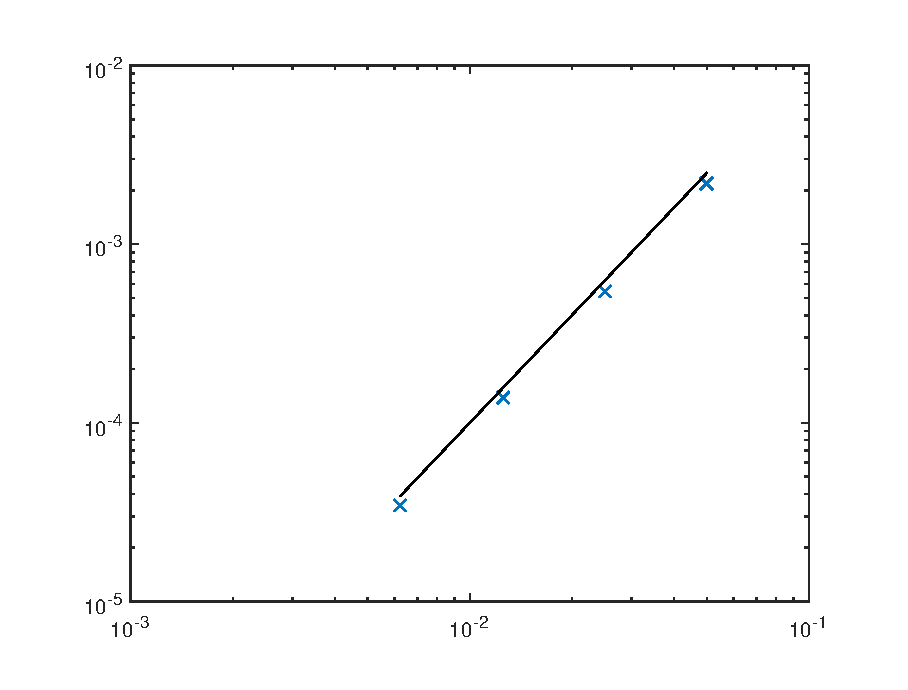
\includegraphics[width=3in]{convStudy}
\caption{loglog plot of error compared with expected error.}
\end{figure}
We can then see that the code presented above converges almost exactly at the rate of $\Delta x^2$.
\pagebreak
\item Use the fact that 
\bq \frac{u_j^{n+1}-2u_j^n+u_j^{n-1}}{\Delta t^2}=(u_{tt})_j^n+\frac{\Delta t^2}{12}(u_{tttt})_j^n+O(\Delta t^4)\eq
as well as the PDE to derive and implement a 4th order accurate code for this problem.\\

Solution:\\

The code I developed is presented here. This code can be run by using the previous run code.
\begin{lstlisting}
function [dx,err] = waveWithSourceO4( N,xa,xb,c,tf,iPlot )
  %N = 50;
  %xa = 0;
  %xb = 1;
  %c = 1;
  %tf = .7;

  %% number of ghost points
  ng = 2;

  %% grid size and other grid quantities
  dx = (xb-xa)/N;
  dt = 0.9*dx/c;
  Nt = ceil( tf/dt );
  dt = tf/Nt;

  Ntot = N+1+2*ng;

  %% first and last interior grid points
  ia = ng+1;
  ib = Ntot-ng;

  x = linspace( xa-ng*dx, xb+ng*dx, Ntot );

[unm1,un] = setICs( x,ia,ib,dx,dt,c);
  
  %% allocate space for u
  u = zeros(size(un));

  if( iPlot == 1 )
    figure
  end

  %% Loop through time
  t = dt;
  for n = 1:Nt-1


    %% set BCs on un
    un = setBCs( un,x,ia,ib,dx,dt,t,c );

    %% compute update over domain interior
    for i = ia:ib
        
        uxx = (-un(i-2)+16*un(i-1)-30*un(i)+16*un(i+1)-un(i+2))/(12*dx^2);
        utt=c^2*uxx+h(x(i),t);
        
        uxxxx=(un(i-2)-4*un(i-1)+6*un(i)-4*un(i+1)+un(i+2))/(dx^4);
        %hxx=-4*h(x(i),t);
        %htt=-h(x(i),t);
        %hxx=(h(x(i-1),t)-2*h(x(i),t)+h(x(i+1),t))/dx^2;
        hxx=(-h(x(i-2),t)+16*h(x(i-1),t)-30*h(x(i),t)+16*h(x(i+1),t)-h(x(i+2),t))/(12*dx^2);
        %htt=(h(x(i),t-1)-2*h(x(i),t)+h(x(i),t+1))/dt^2;
        htt=(-h(x(i),t-2*dt)+16*h(x(i),t-1*dt)-30*h(x(i),t)+16*h(x(i),t+1*dt)-h(x(i),t+2*dt))/(12*dx^2);
        utttt=uxxxx+hxx+htt;
%  utt=-uex(x(i),t,c);
%  utttt=uex(x(i),t,c);
      
        u(i) = 2*un(i)-unm1(i)+dt^2*utt+dt^4*utttt/12;

    end


    %% update solution histories
    unm1 = un;
    un   = u;
    t = t+dt;
    
    if( iPlot == 1 )
      plotStuff( x,u,ia,ib,t,c );
    end
  end
    
  ue = uex( x,t,c );

  ind = ia:ib;
  err = max(abs(u(ind)-ue(ind)));
  return
end

function un = setBCs( un,x,ia,ib,dx,dt,t,c)
  

%     un(ia-1)=cos(2*x(ia-1))*cos(t);
%     un(ia-2)=cos(2*x(ia-2))*cos(t);
%     un(ib+1)=cos(2*x(ib+1))*cos(t);
%     un(ib+2)=cos(2*x(ib+2))*cos(t);
    gltt=(-gl(t-2*dt)+16*gl(t-dt)-30*gl(t)+16*gl(t+dt)-gl(t+2*dt))/(12*dt^2);
    gltttt=(gl(t-2*dt)-4*gl(t-dt)+6*gl(t)-4*gl(t+dt)+gl(t+2*dt))/dt^4;
    htt=(h(x(ia),t-dt)-2*h(x(ia),t)+h(x(ia),t+dt))/dt^2;
    hxx=(h(x(ia-1),t)-2*h(x(ia),t)+h(x(ia+1),t))/dx^2;
    un(ia-1) = 2*un(ia)-un(ia+1)...
            +dx^2*(gltt-h(x(ia),t))...
            +dx^4/(12)*(gltttt-htt-hxx);
            
    un(ia-2)=4*un(ia-1)-6*un(ia)+4*un(ia+1)-un(ia+2)...
            +dx^4*(gltttt-htt-hxx);
        
    grtt=(-gr(t-2*dt)+16*gr(t-dt)-30*gr(t)+16*gr(t+dt)-gr(t+2*dt))/(12*dt^2);
    hx=(h(x(ib+1),t)-h(x(ib-1),t))/(2*dx);
    
    un(ib+1) = un(ib-1)+dx^3/3*(grtt-hx)+2*dx*gr(t);
    un(ib+2) = 2*un(ib+1)-2*un(ib-1)+un(ib-2)+2*dx^3*(grtt-hx);
%     un(ib)=gr(t);
%     un(ia)=gl(t);
  return
end

function z = uex( x,t,c )
  z = cos(2*x)*cos(t);
  return
end

function z = f( x )
  %% solution at t=0
  z = cos(2*x);
  return
end

function z = g( x )
  %% time derivative of solution at t=0
  z = 0;
  return
end

function z = h( x,t )
    %% Source term
    z = 3*cos(2*x)*cos(t);
    return
end

function z=gl(t)
z=cos(t);
return
end

function z=gr(t)
z=-2*sin(2)*cos(t);
return
end

function plotStuff( x,u,ia,ib,t,c )

  ue = uex( x,t,c );

  ind = ia:ib;
  subplot( 2,1,1 )
  plot( x(ind),u(ind),'rx', x(ind),ue(ind),'k-' );
  xlabel( 'x' );
  ylabel( 'u' );

  subplot(2,1,2)
  plot( x(ind),u(ind)-ue(ind),'rx' );
  xlabel( 'x' );
  ylabel( 'error' );
  drawnow;
  pause
  
  return
end

function [unm1,un] = setICs( x,ia,ib,dx,dt,c )
  %% set intial condition at t=0 (and then BCs on initial condition)
  unm1 = zeros(size(x));
  for i = ia:ib
    unm1(i) = f( x(i) );
  end
  unm1 = setBCs( unm1,x,ia,ib,dx,dt,0,c );
  
  %% now set initial condition at t=dt (and then BCs)
  %% here we use a Taylor expansion in time
  un = zeros(size(x));
  for i = ia:ib
    fm2 = f(x(i-2));
    fm1 = f(x(i-1));
    f0  = f(x(i));
    fp1 = f(x(i+1));
    fp2 = f(x(i+2));
    
    g0  = g(x(i));
    hm1=h(x(i-1),0);
    htm1=h(x(i),-dt);
    h0  = h(x(i),0);
    hp1=h(x(i+1),0);
    htp1=h(x(i),dt);
    
    
    uxx = (-fm2+16*fm1-30*f0+16*fp1-fp2)/(12*dx^2);
    
    utt = c^2*uxx+h0;
    
    
    uttt=(htp1-htm1)/(2*dt);
    
    uxxxx= (fm2-4*fm1+6*f0-4*fp1+fp2)/dx^4;
    hxx= (hm1-2*h0+hp1)/dx^2;
    htt= (htm1-2*h0+htp1)/dt^2;
    
    utttt=uxxxx+hxx+htt;

    %utt=-uex(x(i),dt,c);
    %utttt=uex(x(i),dt,c);
    %uttt=-cos(2*x(i))*sin(dt);
    
    un(i) = f0+0.5*dt^2*(utt)+dt^3/6*uttt+dt^4/24*utttt;
%un(i)=uex(x(i),dt,c);

  end
  un = setBCs( un,x,ia,ib,dx,dt,dt );
  return
end
\end{lstlisting}
A convergence analysis was run to determine that this code actually runs at 4th order accuracy. The code use to generate the result is presented here, immediately below the result. We see that the code is slightly faster than 4th order accurate. Interestingly enough, the biggest barrier to reaching 4th order accuracy is in finding an appropriate discretization of $h_{tt}(x,t)$ where it appears in the time stepping loop. With a discrete definition of the derivative, the best I could acheive was 2nd order accuracy. But with an analytic definition of the derivative the code is 4th order accurate as we see here.

\begin{figure}[h]
\centering
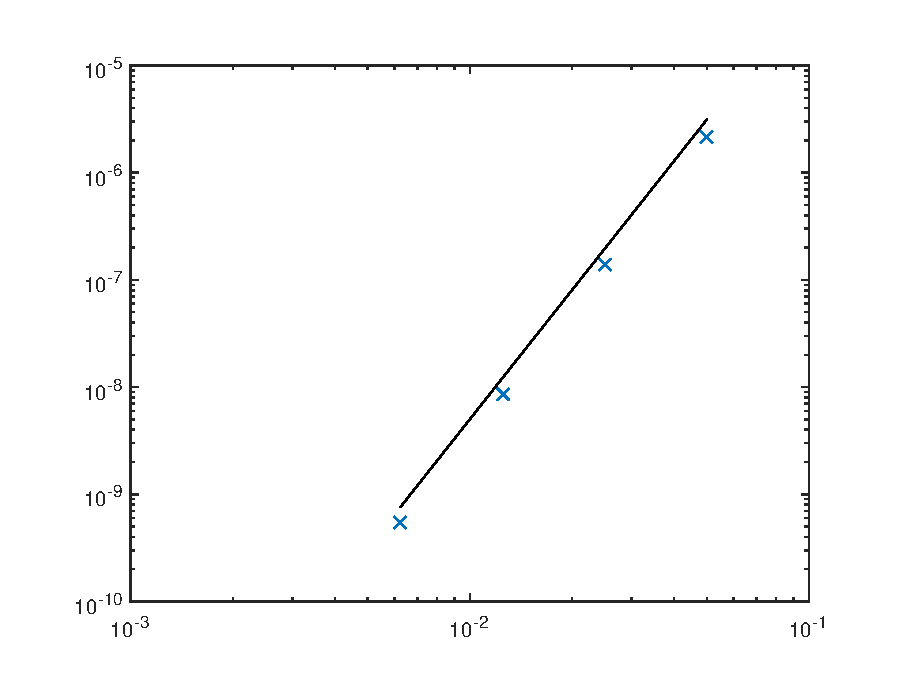
\includegraphics[width=3in]{convStudyO4}
\end{figure}
\begin{lstlisting}
N0 = 20;

xa = 0;
xb = 1;
c = 1;
tf = 1;
m = 4;

hPlot   = zeros(m,1);
errPlot = zeros(m,1);

for k = 0:m-1
  N = N0*2^k;  
  [hPlot(k+1),errPlot(k+1)] = waveWithSourceO4( N,xa,xb,c,tf,0);
end

loglog( hPlot,errPlot,'x', hPlot,(hPlot.^4)/2, 'k-' );
\end{lstlisting}
\eenum
\eenum
\end{document}


















